
\chapter{Use Cases} \label{use_cases}

The main purpose of the current chapter is to demonstrate the functionalities of the web platform, by building analysis pipelines using real data from the literature. For this, two distinct datasets were used. The first use case is the discrimination of propolis samples from southern Brazil according to chemical profile (using \gls{uv} data) \citep{tomazzoli2015discrimination}, while the second use case consists in the chemical and enzymatic composition screening in several genotypes of cassava roots during \gls{ppd} (using \gls{ir} data) \citep{uarrota2014metabolomics}.


\section{Propolis}

\subsection{Context}

The propolis resinous substance is collected by honeybees \textit{Apis mellifera} from various plant sources and added to salivary enzymes, beeswax, and pollen. They use it to seal openings and for protection against microorganisms and insects.

However, this substance also offers a broad spectrum of biological activities, including, for instance, cytotoxic, anti-herpes, free radical scavenging, antimicrobial, and anti-HIV activities, being used in both cosmetic and pharmaceutical markets. Therefore, the botanical origin of propolis is extremely important to guarantee raw materials of superior quality are supplied to said markets.

Since propolis quality depends, among other variables, on the local flora
which is strongly influenced by (a)biotic factors over the seasons, the main scope of the study was to determine the harvest season effect on the chemical profile of this substance.

For this, propolis samples from \textit{A. mellifera} were collected in Southern Brazil throughout 2014, and samples visually classified according to their color. The \gls{uv} absorbance values were recorded using a spectral window of 280-800 $\eta m$.


\subsection{Data Overview}

In \autoref{propolis_data_overview} the propolis dataset summary and metadata table is shown. The \gls{uv} dataset has no missing values, 5 metadata variables, a total of 165 samples and 521 data points. The last column of the metadata table (replicates) was omitted for formating reasons.

\begin{figure}[h]
	\centering
	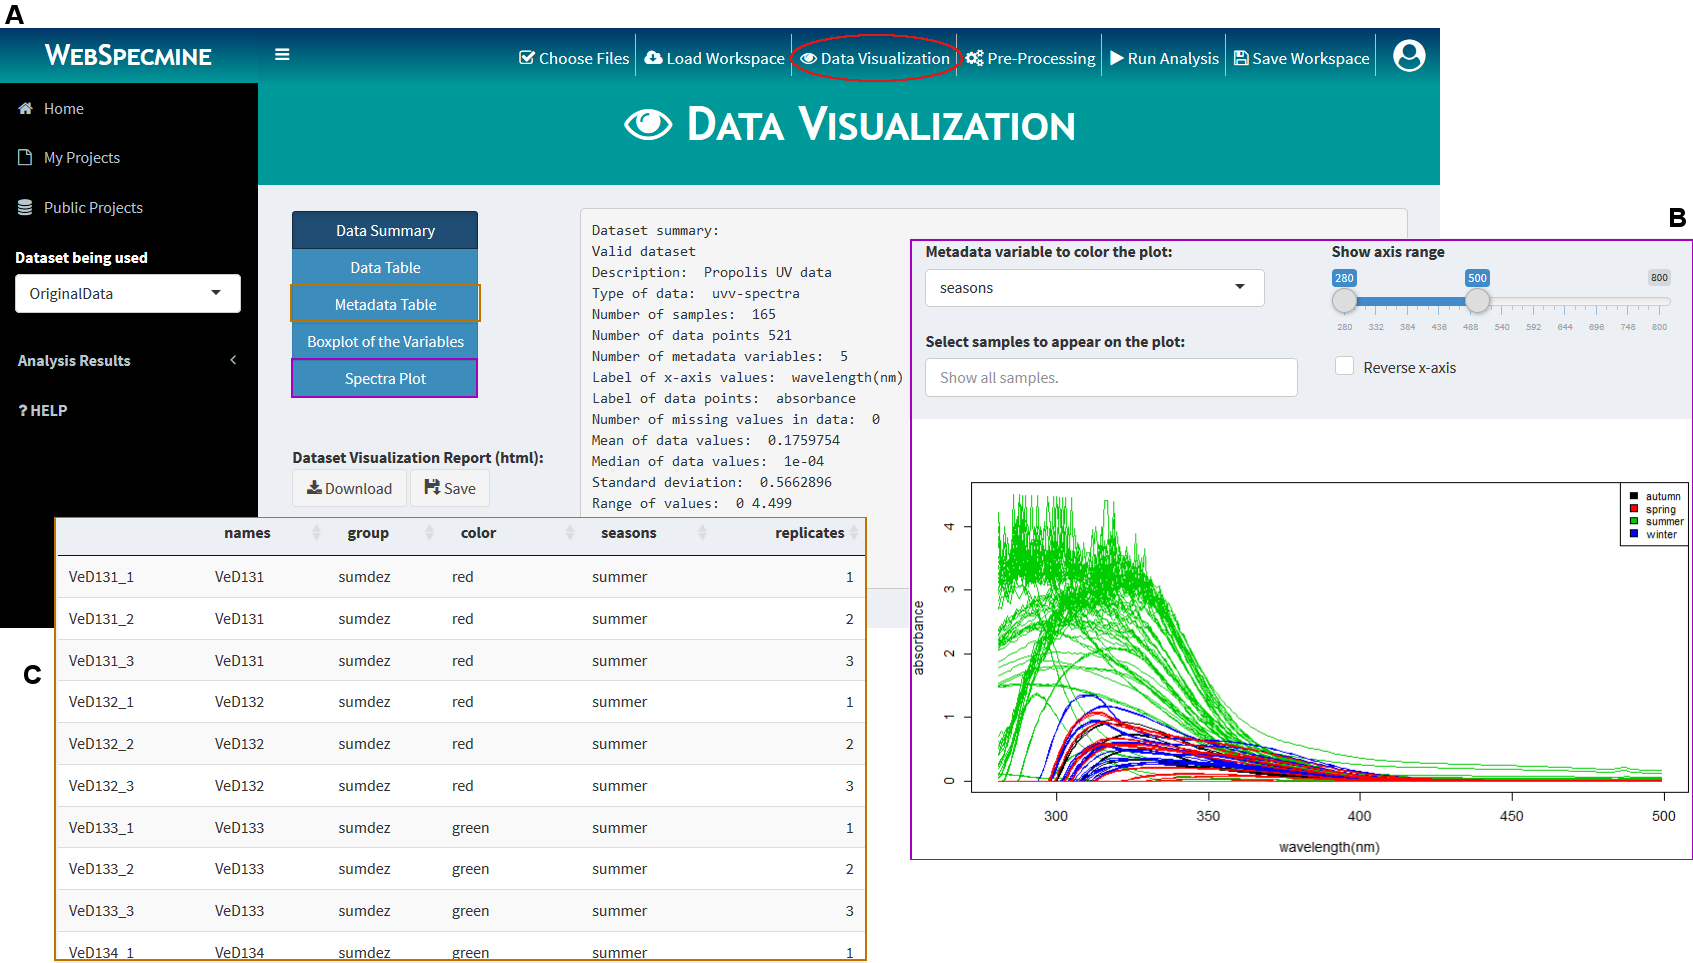
\includegraphics[width=1\linewidth]{Imagens/Propolis/data_overview}
	\caption{The dataset summary (\textbf{A}) and partial metadata table (\textbf{B}).}
	\label{propolis_data_overview}
\end{figure}


\subsection{Preprocessing}

Smoothing interpolation was initially performed over the propolis dataset, followed by background, offset and baseline corrections (\autoref{propolis_spectra}). 

\begin{figure}[h]
	\centering
	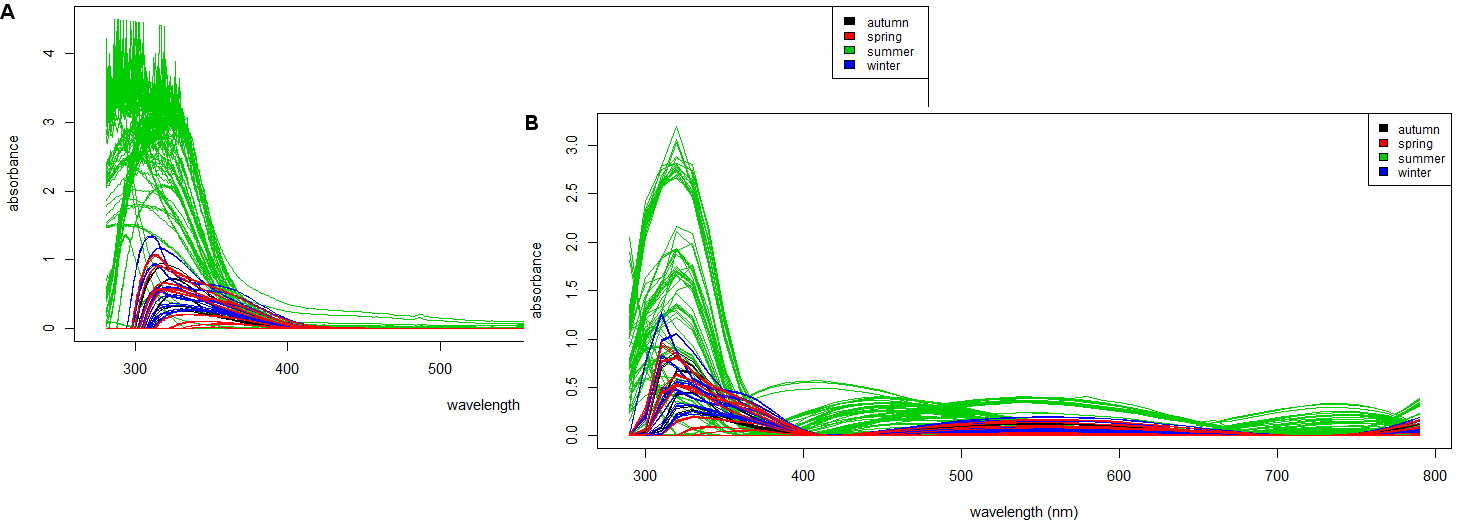
\includegraphics[width=1\linewidth]{Imagens/Propolis/spectra}
	\caption{Propolis raw spectra (\textbf{A}) and spectra processed with smoothing interpolation, background, offset and baseline corrections (\textbf{B}), with samples colored according to season.}
	\label{propolis_spectra}
\end{figure}


\subsection{Univariate Analysis}





\subsection{Clustering}

An \acrlong{hca} with Euclidean distance measure and complete agglomeration method was performed over the propolis dataset. Samples were discriminated in two groups, the first one having samples collected in the four seasons and the second containing almost exclusively propolis samples produced in the summer.

\begin{figure}[h]
	\centering
	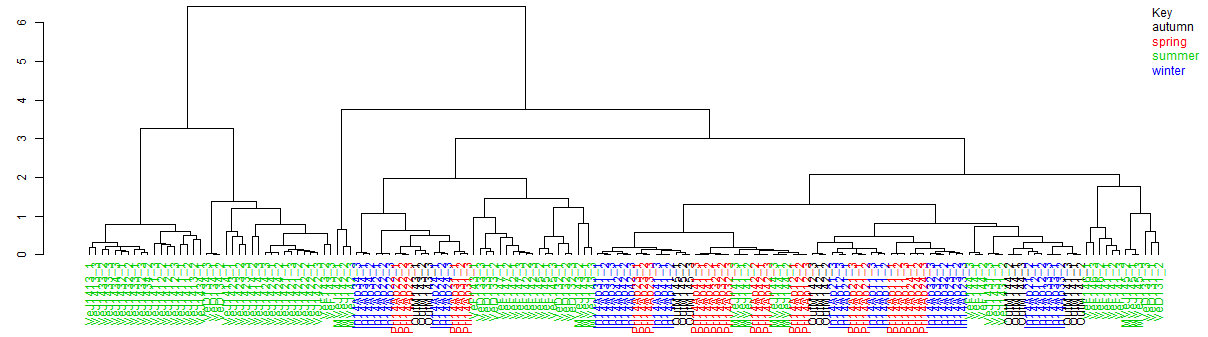
\includegraphics[width=1\linewidth]{Imagens/Propolis/hca}
	\caption{Hierarchical clustering analysis dendrogram of the propolis dataset. Euclidean distance and a complete agglomeration method were used.}
	\label{propolis_hca}
\end{figure}


\subsection{Principal Components Analysis}

A robust \gls{pca} was also performed, using data centered (by mean) and scaled (by standard deviation method) (\autoref{propolis_pca}). With the first and second components explaining 49.9\% and 25.0\% of total variance, respectively, this results have confirmed the sample discrimination by seasons into two groups, as observed in the \gls{hca} (\autoref{propolis_pca_scores2D}).

\begin{figure}[h]
	\centering
	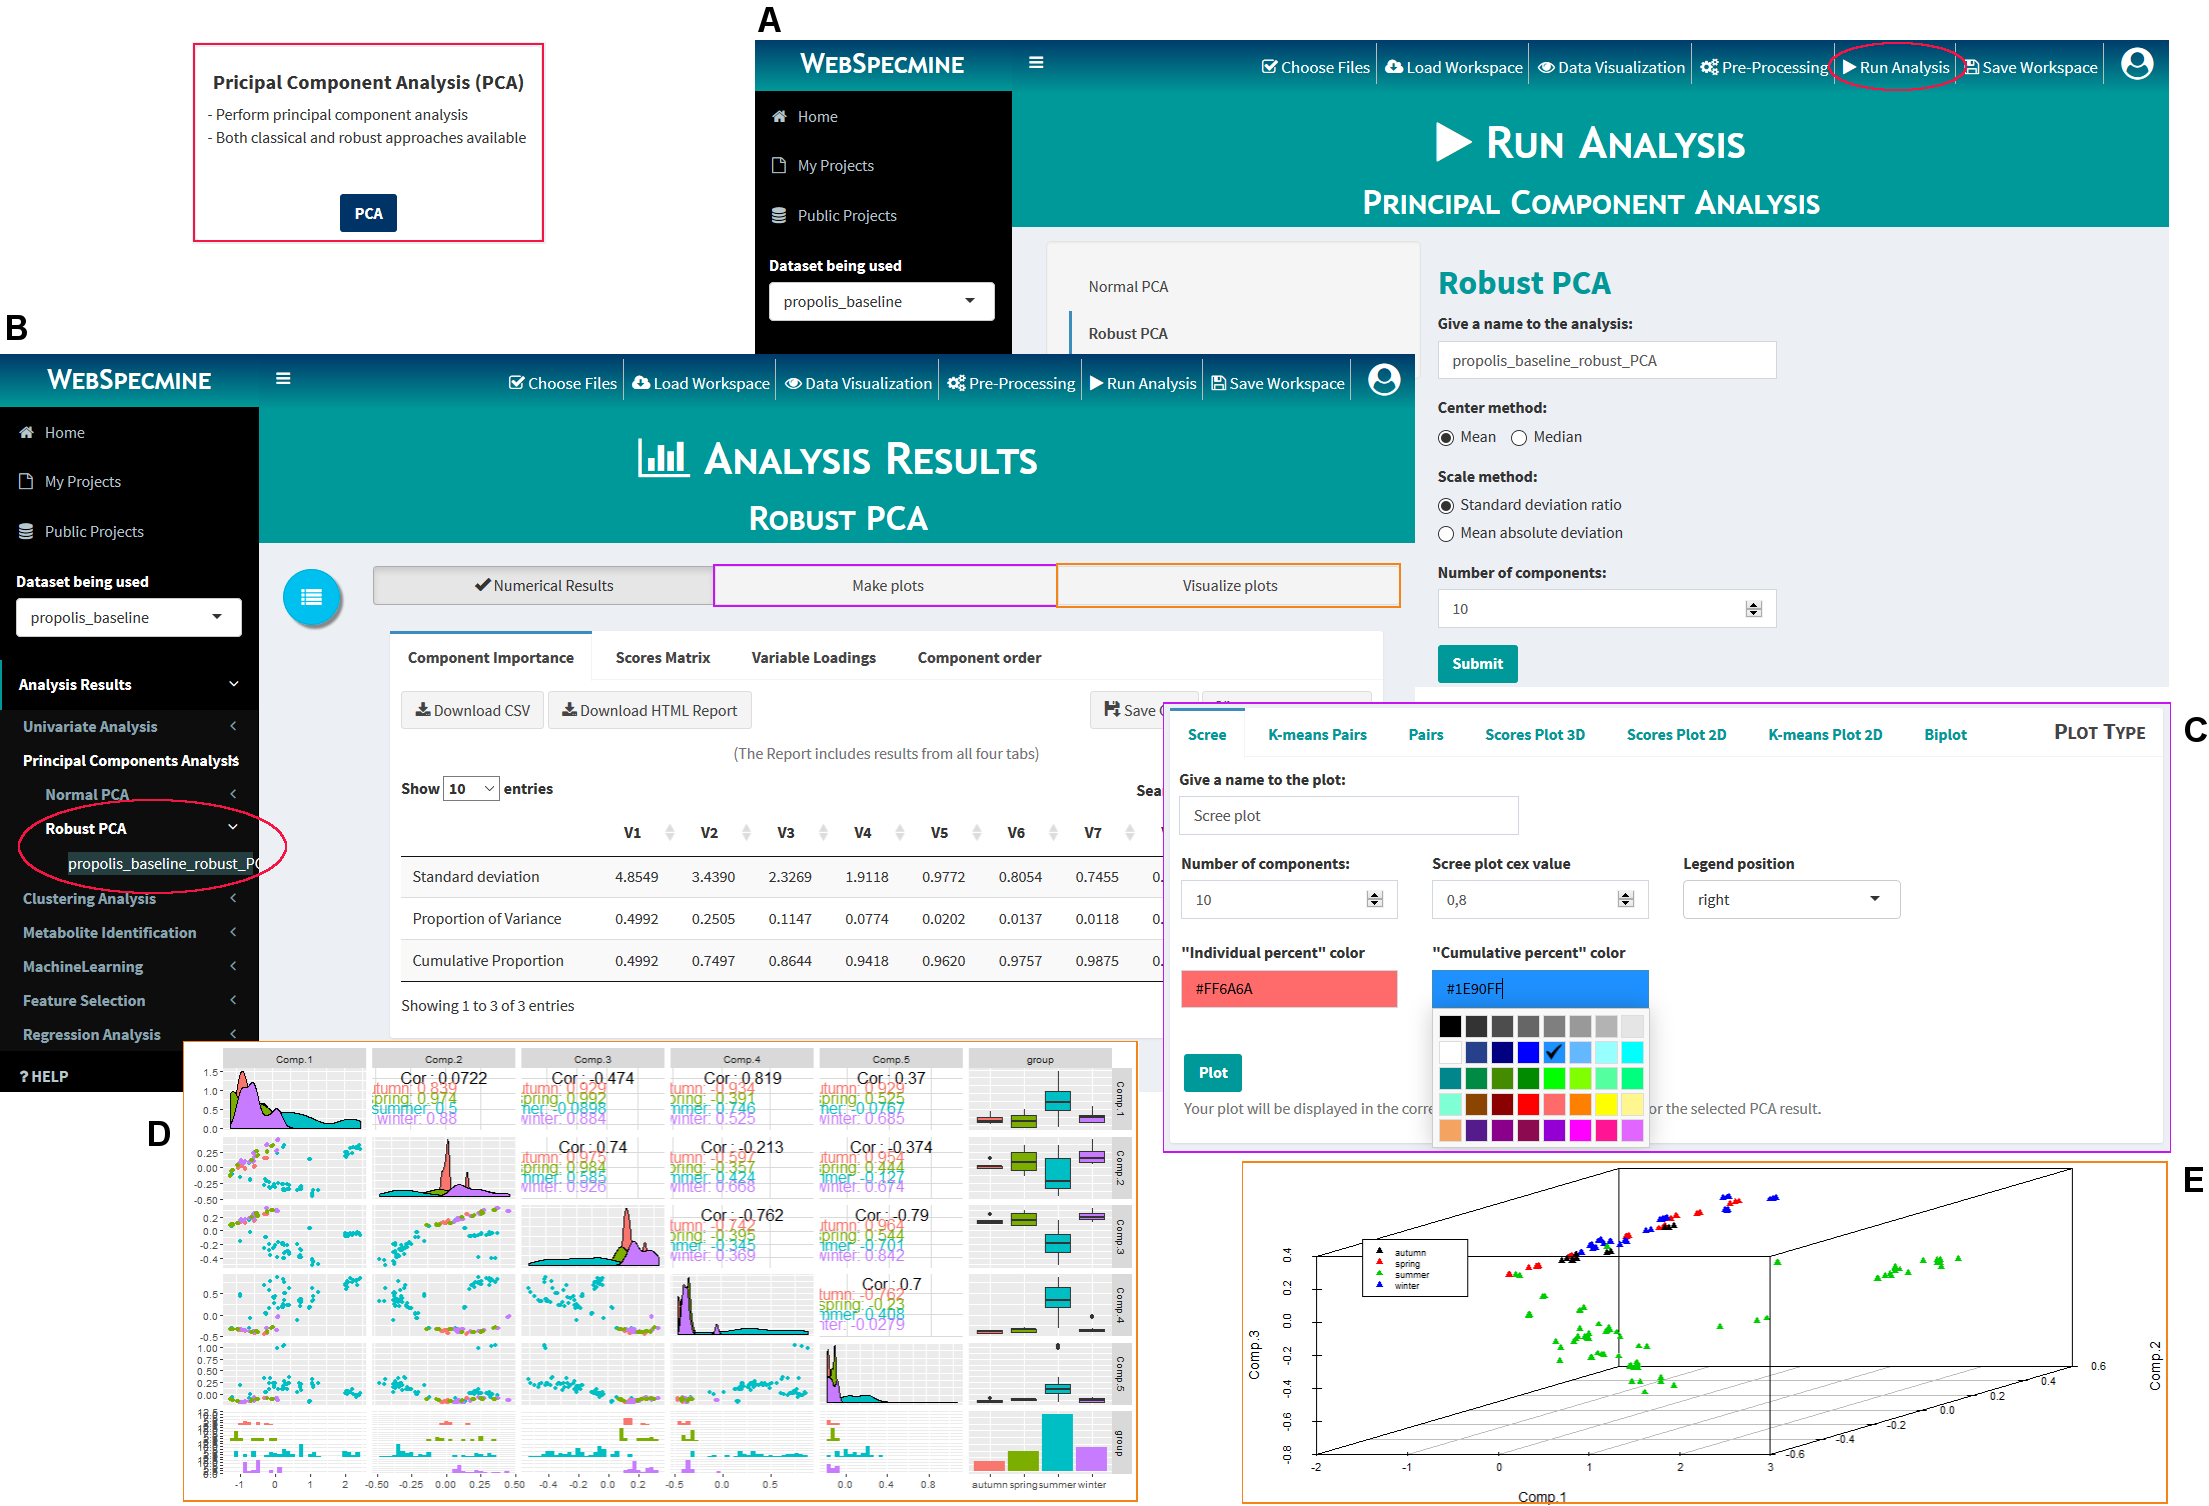
\includegraphics[width=1\linewidth]{Imagens/Propolis/pca}
	\caption{Principal components importance (\textbf{A}) and variable loadings (\textbf{B}) tables from the \gls{pca} performed over the propolis dataset.}
	\label{propolis_pca}
\end{figure}


\begin{figure}[h]
	\centering
	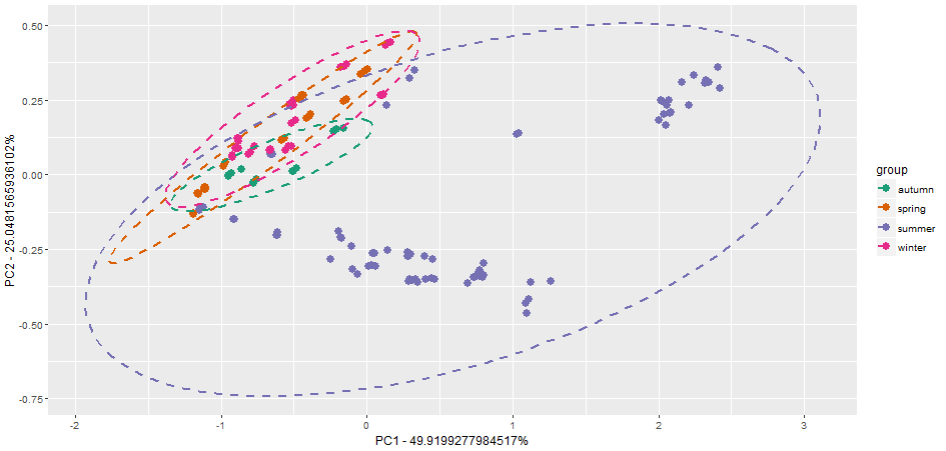
\includegraphics[width=1\linewidth]{Imagens/Propolis/pca_scores2D}
	\caption{Scores scatter plot of the \gls{pca} performed over the propolis dataset for the first and second components.}
	\label{propolis_pca_scores2D}
\end{figure}











